\let\negmedspace\undefined
\let\negthickspace\undefined
\documentclass[journal]{IEEEtran}
\usepackage[a5paper, margin=10mm, onecolumn]{geometry}
%\usepackage{lmodern} % Ensure lmodern is loaded for pdflatex
\usepackage{tfrupee} % Include tfrupee package

\setlength{\headheight}{1cm} % Set the height of the header box
\setlength{\headsep}{0mm}     % Set the distance between the header box and the top of the text

\usepackage{gvv-book}
\usepackage{gvv}
\usepackage{cite}
\usepackage{amsmath,amssymb,amsfonts,amsthm}
\usepackage{algorithmic}
\usepackage{graphicx}
\usepackage{textcomp}
\usepackage{xcolor}
\usepackage{txfonts}
\usepackage{listings}
\usepackage{enumitem}
\usepackage{mathtools}
\usepackage{gensymb}
\usepackage{comment}
\usepackage[breaklinks=true]{hyperref}
\usepackage{tkz-euclide} 
\usepackage{listings}
% \usepackage{gvv}                                        
\def\inputGnumericTable{}                                 
\usepackage[latin1]{inputenc}                                
\usepackage{color}                                            
\usepackage{array}                                            
\usepackage{longtable}                                       
\usepackage{calc}                                             
\usepackage{multirow}                                         
\usepackage{hhline}                                           
\usepackage{ifthen}                                           
\usepackage{lscape}
\usepackage{circuitikz}
\tikzstyle{block} = [rectangle, draw, fill=blue!20, 
    text width=4em, text centered, rounded corners, minimum height=3em]
\tikzstyle{sum} = [draw, fill=blue!10, circle, minimum size=1cm, node distance=1.5cm]
\tikzstyle{input} = [coordinate]
\tikzstyle{output} = [coordinate]


\begin{document}

\bibliographystyle{IEEEtran}
\vspace{3cm}

\title{4.2.4}
\author{EE25BTECH11001 - Aarush Dilawri}
\maketitle
% \newpage
% \bigskip
{\let\newpage\relax\maketitle}

\renewcommand{\thefigure}{\theenumi}
\renewcommand{\thetable}{\theenumi}
\setlength{\intextsep}{10pt} % Space between text and floats


\numberwithin{equation}{enumi}
\numberwithin{figure}{enumi}
\renewcommand{\thetable}{\theenumi}

\textbf{Question}:\\
Find the direction and normal vector for the line 
\begin{align}
x = 3y
\end{align}
\solution \\

The line can be written as: 
\begin{align}
x - 3y =0
\end{align}

This equation can be expressed in terms of matrices\\
Let
\begin{align}
\vec{x} = \myvec{x \\ y}
\end{align}
\begin{align}
\vec{n^T} = \myvec{1 & -3}
\end{align}
\begin{align}
c = 0
\end{align}

The line equation can be written as:
\begin{align}
\vec{n^T}  \vec{x} = c
\end{align}

Where $\vec{n}$ is the normal vector of the given line

The direction vector of the line can be found by observing the normal vector.
\begin{align}
\vec{m} = \myvec{3 \\ 1}
\end{align}


This is true because if the director vector is represented as 
\begin{align}
\vec{m}  = \myvec{1 \\ m}    
\end{align}
then the normal vector can be represented as 
\begin{align}
\vec{n} = \myvec{-m \\ 1}
\end{align}

This can be verified by the following equation:
\begin{align}
\vec{n^T}\vec{m} = 0
\end{align}

\begin{align}
\myvec{1 & -3}\myvec{3 \\ 1} = 0
\end{align}\\



The normal vector of the line is $\vec{n} = \myvec{1 \\ -3}$
The director vector of the line is $\vec{m} = \myvec{3 \\ 1}$\\

From the figure, it is clearly verified that the theoretical solution matches with the computational solution.\\
\begin{figure}[h!]
    \centering
    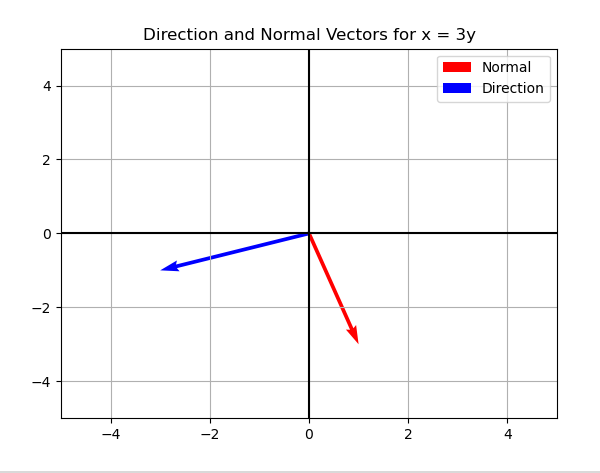
\includegraphics[height=0.5\textheight, keepaspectratio]{figs/fig.png}
    \label{figure_1}
\end{figure}

\end{document}